\chapter{Równania Lotki-Volterry dla konkurencji}

\section{Model matematyczny}

\noindent Rozważając temat modelowania populacji za pomocą równań logistycznych warto poruszyć temat modelów uwzględniających również konkurencję o pożywienie i ogólnie system z wielogatunkowymi poziomami troficznymi.

\noindent W odpowiedzi przychodzi układ równań w formie podobnej do klasycznych, modelujących relacje ofiara-drapieżnik. Oparte są na bazie równań logistycznych postaci $\frac{d}{dx}f(x) = f(x)(1-f(x))$.  W przypadku standardowego układu Lotki-Volterry przypadkiem bazowym był wzrost wykładniczy.

\noindent Przypadek zająca i owcy mógłby zostać opisany następującym układem równań:

$$\frac{dN_1}{dt}=N_{1}r_{1}\left(1-\frac{\left({N_{1}+\alpha _{{12}}N_{2}}\right)}{K_1}\right)$$
$$\frac{dN_2}{dt}=N_{2}r_{2}\left(1-\frac{\left({N_{2}+\alpha _{{21}}N_{1}}\right)}{K_2}\right)$$

\begin{eqwhere}[2cm]
	\item[$r_1,r_2$] wzrost per capita członków poszczególnych populacji 
	\item[$\alpha_{nm}$] współczynnik konkurencji jednostki z populacji $m$ na jednostkę z populacji $n$
	\item[$K_1,K_2$] zdolność pojemnościowa układu dla poszczególnych populacji
\end{eqwhere}

\noindent Założeniem logistycznego modelu jest to, że liczba potomstwa per rodzic maleje liniowo ze wzrostem populacji tej populacji.

\noindent Włączając w to konkurencję innego gatunku, liczba potomstwa na rodzica zależy nie tylko od populacji pierwszej, ale również od populacji drugiej.

\newpage

\begin{figure}
	\centering
	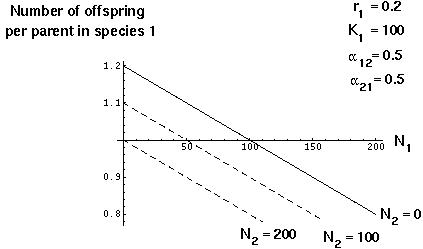
\includegraphics[width=\textwidth]{img/Fig1}
	\caption{Liczba potomków na dorosłego osobnika w funkcji parametrów}
\end{figure}

\section{Właściwości modelu}

\begin{itemize}[itemsep=0em]
	\item jeśli $\alpha_{12}$ wynosi zero, wtedy dynamika gatunku pierwszego będzie przedstawiona równaniem logistycznym (sigmoidalny wykres) 
	
	\item analagicznie dla $\alpha_{21} = 0$
	
	\item jeśli $\alpha_{12} < 0$ to populacja druga zwiększa liczbę surowców dostępnych dla populacji pierwszej
	
	\item jeśli oba współczynniki $\alpha_{12},\alpha_{21} = 0$ to relację między populacjami nazywamy mutualizmem
	
	\item jeśli $\alpha_{12}$ albo $\alpha_{21}$ jest równe zero (albo bardzo blisko zera), to mówimy że populacje są w relacji komensalizmu
	
	\item jeśli tylko jeden ze współczynników jest ujemny, a drugi dodatni, to mówimy, że populacje są w relacji pasożytnictwa
	
	\item jeśli oba współczynniki są dodatnie to populacje ze sobą konkurują
	
\end{itemize}

\section{Symulacje dla dodatnich współczynników}

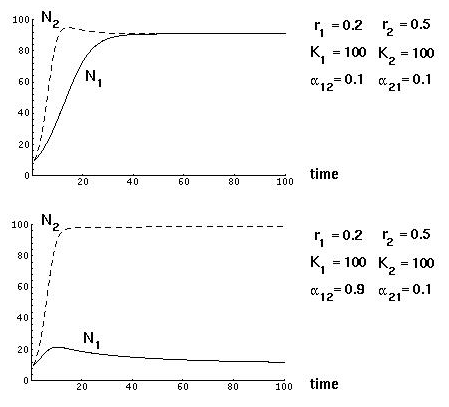
\includegraphics{img/Fig2}

\noindent Jeśli $\alpha_{12}$ i $\alpha_{21}$ są małe, to obie populacje osiągają ekwilibrium w pobliżu odpowiedniej pojemności systemu. Jeśli $\alpha_{12}$ jest znacznie większe od $\alpha_{21}$ (gatunek drugi ma większy impakt na liczebność gatunku pierwszego niż odwrotnie), wtedy liczebność gatunku pierwszego jest utrzymywana na niskim poziomie spowodowanym wyższością konkurencyjności drugiego gatunku.

\noindent Do stworzenia stabilnego ekosystemu wszyste wartości własne macierzy $a_{ij}$ muszą być dodatnie. Duże systemy Lotki-Volterry mogą osiągnąć stabilność jeśli współczynniki konkurencji $\alpha_{ij}$ mogą ewoluować zgodnie z naturalną selekcją (\cite{Kon} i \cite{Ack})